\documentclass{article}
\renewcommand{\figurename}{Figura}
\renewcommand{\contentsname}{Indice}
\usepackage{float}
\usepackage[utf8x]{inputenc}
\usepackage{algorithm}
\usepackage{algpseudocode}

\usepackage{graphicx}
\usepackage[usenames, dvipsnames]{color}
\usepackage[table]{xcolor}

\usepackage{vmargin}
  %configuración de pagina:
\setpapersize{A4}
\setmargins{2.5cm}       % margen izquierdo
{1.5cm}                  % margen superior
{16.5cm}                 % anchura del texto
{23.42cm}                % altura del texto
{10pt}                   % altura de los encabezados
{1cm}                    % espacio entre el texto y los encabezados
{0pt}                    % altura del pie de página
{2cm}                    % espacio entre el texto y el pie de página


\begin{document}

%quiza podamos cambiar la caratula a la del DC, tipo algo1,algo2
\begin{titlepage}
	\centering
	\vspace{1cm}
	{\normalfont\huge Universidad de Buenos Aires \par}
	\vspace{1cm}
	{\normalfont\Large Facultad de Ciencias Exactas y Naturales\par}
	{\normalfont\Large Departamento de Computación\par}
	\vspace{1.5cm}
	{\bfseries\huge Algoritmos y Estructuras 3 \par}
	\vspace{1.5cm}
	{\normalfont\huge Trabajo Práctico N°1 \par}
	\vspace{1.5cm}
	
	{\large
		\begin{tabular}{l c l}
		Autor & LU & Correo electrónico \\
		\hline
		Carbonelli, Lucas 	& 596/15 & luc92ac@hotmail.com \\
		\end{tabular}
	}
	


\end{titlepage}

\newpage

%habría que hacer que no diga contents en inglés, en métodos no pudimos...
\textbf{\tableofcontents{}}

\newpage

\section{Introducción}

Este trabajo tiene como objetivo mostrar la resolución de un problema en particular, mediante una solución algorítmica que utilice la técnica backtraking.
El problema en cuestión consiste en determinar la confiabilidad de un grupo de agentes utilizando una encuesta que mide la confianza entre los mismos. Los agentes deben opinar sobre cada uno, inclusive ellos mismos.
Como resultado de la encuesta, se obtiene un conjunto de afirmaciones de la forma "X dice que Y es confiable", "X dice que Y no es confiable". Si X es confiable entonces se asume que lo que el agente opina siempre es verdadero. Caso contrario, si X no es confiable, entonces las opiniones pueden ser verdaderas o falsas. Lo que se busca es determinar la máxima cantidad de agentes en los que se puede confiar, de modo que las respuestas a la encuesta sean consistentes. \\
Por ejemplo, si tenemos un conjunto de cuatro informantes A,B,C y D, que responden a la encuesta de la siguiente manera:
\begin{itemize}
	\item A dice que B es confiable
	\item A dice que D no es confiable
	\item B dice C no es confiable
	\item C dice que A son confiables
	\item C dice que D son confiables
\end{itemize}
Se puede confiar en dos agentes como máximo, por ejemplo en los agentes A y B. Cualquier conjunto de tres agentes es inconsistente. Por ejemplo el conjunto que incluye a los agentes A, B y C no es válido porque el B dice que C no es confiable.\\
En síntesis, un conjunto es válido si cumple las siguientes condiciones:
\begin{itemize}
	\item Ningún agente en el conjunto diga que es confiable un agente que no esta en el conjunto.
	\item Ningún agente en el conjunto diga que no es confiable un agente en el conjunto.
\end{itemize}

La entrada del programa que resuelve este problema consiste de varios casos que se procesan en lote. Cada caso comienza con dos enteros no negativos $1 \leq i$ y $0 \leq a$, separados por espacios en blancos. $i$ es el número de informantes y $a$ es el número de respuestas a encuestas. Luego hay $a$ líneas, cada una con dos números $x$ y $y$ ($1 \leq x \leq i, 1 \leq |y| \leq i$) separados por espacios en blanco. Si $y$ es positivo, la línea de entrada significa que el agente "$x$ dice que el agente $y$ es confiable". Si $y$ es negativo entonces, la línea de entrada significa que el agente "$x$ dice que el agente $-y$ no es confiable". El final de la entrada se indica con una línea con dos ceros. Por cada caso de entrada escribir en la salida una línea con la máxima cantidad de agentes. Por ejemplo, dada la siguiente entrada: \\
4 5 \\
1 2 \\
1 -4 \\
2 -3 \\
3 1 \\
3 4 \\
1 1 \\
1 -1 \\
3 3 \\
1 2 \\
2 3 \\
3 -1 \\
0 0 \\ \\
El programa devuelve: \\
2 \\
0 \\
2 \\

La técnica backtraking consiste en ir creando todas las posibles soluciones (en este caso particular, conjuntos de agentes), y analizar su validez. La ventaja de esta técnica es que se vale de las restricciones del problema para evitar analizar conjuntos de soluciones invalidas, reduciendo el tiempo de ejecución. Cada sección del algoritmo que permite reducir el conjunto de soluciones se denomina poda. El algoritmo planteado implementa dos podas. El la sección de resultados se detallan las pruebas realizadas para medir el impacto de cada poda por separado y combinadas.
En la sección Implementación se presenta el algoritmo y se deduce su complejidad, la cual es $O(2^i i^2 a^2) $.
 El algoritmo se implementó en C++. 

\section{Implementación}

\subsection{Pseudocódigo}

El pseudocodigo del algoritmo implementado se muestra a continuación:

\begin{algorithm}
\begin{algorithmic}[1]
\Function{cantidadAgentesConfiablesBT}{conjAgentesSolución,listaOpiniones}
\For{$c \in$ conjAgentesSolución} \Comment{$O(i)$}
	\For{$l \in$ listaOpiniones} \Comment{$O(a)$}
		\If{$c$ opina de otro agente en conjAgentesSolución} \Comment{Buscar al agente en el conj $O(i)$}
			\State $c$ opina sobre $c'$, $c' \in$ conjAgentesSolución				\EndIf
		\If{opinión de $c$ sobre $c'$ invalida el conjunto} \Comment{$O(1)$}
			\State Se descarta toda la rama
		\EndIf

			\If{$c'$ no está en conjAgentesSolución AND $c$ confía en $c'$} \Comment{$O(1)$}
				\If{Algún agente dice que $c'$ no es confiable} \Comment{Buscar al agente en las opiniones $O(a)$}				
					\If{Es un agente de la solución} \Comment{Buscar al agente en el conj $O(i)$}
						\State Se poda la rama \Comment{Poda A $O(1)$}			
					\EndIf
				\EndIf
			\EndIf
	\EndFor
\EndFor
\State agentesConfiablesHastaAhora $\gets$ conjAgentesSolución.tam \Comment{$O(1)$}
\For{$c \in$ conjAgentesSolución.ultimo+1,i} \Comment{$O(i)$}
	\If{No quedan agentes para armar un conjunto mayor a agentesConfiablesHastaAhora} 
		\State Se poda la rama \Comment{Poda B $O(1)$}
	\EndIf
	\State conjAgentesSolución.agregar($c$) \Comment{$O(1)$}
	\State agentesConfiablesTmp $\gets$ cantidadAgentesConfiablesBT(conjAgentesSolución,listaOpiniones)
	\If{agentesConfiablesTmp $>$ agentesConfiablesHastaAhora} \Comment{$O(1)$}
		\State agentesConfiablesHastaAhora $\gets$ agentesConfiablesTmp \Comment{$O(1)$}
	\EndIf
	\State conjAgentesSolución.eliminar($c$) \Comment{$O(1)$}
\EndFor
\If{agentesConfiablesHastaAhora $==$ conjAgentesSolución.tam} \Comment{$O(1)$}
	\If{Agente Y no esta en el conjunto, X confia en Y} \Comment{$O(i^2*a)$}
		\State Se descarta toda la rama
	\EndIf
\EndIf
\EndFunction
\end{algorithmic}
\end{algorithm}


Este algoritmo puede dividirse en tres partes. En la primera parte se verifica la consistencia del conjunto y se evalúa si puede realizarse una de las podas. En la segunda, se efectúa la llamada recursiva y se evalúa si puede realizarse la otra poda. Finalmente, en la tercera parte se verifica una de las condiciones en una situación que no podía evaluarse con anterioridad. \\
Cabe recordar que hay $i$ agentes y $a$ respuestas u opiniones. Los agentes internamente se almacenan como números del 1 al $i$. La solución que se está analizando en un momento dado se guarda en conjAgentesSolución, que es un conjunto ordenado de agentes. Está implementado como un vector en C++. El orden se mantiene debido a la forma en que se insertan y eliminan los elementos del vector, siempre el elemento que se inserta es mayor al último elemento del vector y se lo agrega al final del mismo.

\subsection{Complejidad}

El algoritmo está dividido en tres partes que se ejecutan en serie, por lo tanto se suman sus complejidades. La primera parte tiene dos ciclos exterior con complejidades $O(i)$ y $O(a)$. En el interior tiene un ciclo con complejidad $O(i)$ y otros dos ciclos anidados con complejidad total $O(a i)$. En total la primera parte tiene complejidad $O(i a (a i + a)) = O(i^2 a^2)$.
La segunda parte itera a través de los agentes, por lo tanto, tiene complejidad $O(i)$.
La tercera parte es análoga a la primera pero sin el doble ciclo anidado interno, es $O(i^2 a)$. Finalmente, cada llamada recursiva tiene complejidad $O(i^2 a^2)$ + $O(i)$ + $O(i^2 a)$ = $O(i^2 a^2)$.
En la segunda parte del algoritmo, hace llamadas recursivas de forma iterativa de forma tal de generar, en el peor de los casos, tantas llamadas como subconjuntos de un conjuntos de $i$ hay. En un conjunto de $i$ elementos hay $P(i) = 2^i$ subconjuntos, por lo tanto, la complejidad del algoritmo es $O(2^i i^2 a^2)$

\subsection{Análisis del algoritmo}

En la primera parte se analiza la validez del conjunto de agentes, verificando las siguientes inconsistencias:

\begin{enumerate}
	\item Los agentes X e Y están en el conjunto pero X no confiá en Y
	\item El agente X está en el conjunto pero el agente Y no. X confiá en Y. Agente Y es menor al ultimo agente X agregado.
\end{enumerate}

En caso de encontrarse alguna de las inconsistencias anteriores, la rama se descarta inmediatamente. Vale destacar que la inconsistencia 2 tiene sentido debido a la forma en que se agregan los agentes, detallada anteriormente. \\
En esta parte también se evalúa la primera poda (poda A desde ahora). Esta poda intenta predecir si eventualmente al explorar la rama actual se desembocará en un conjunto inconsistente. La comprobación que realiza se puede sintetizar de la siguiente manera: "Si el agente Y no está en el conjunto, pero dentro del conjunto hay un agente que dice que es confiable y otro que dice que no, eventualmente el conjunto será considerado invalido." \\
Luego, en la segunda parte del algoritmo se efectúa la llamada recursiva. En una variable se guarda el tamaño del conjunto válido más grande encontrado hasta el momento. Luego se itera por el conjunto de agentes que son mayores al que había sido agregado en la instancia inmediatamente superior del árbol de recursión. En cada iteración se agrega el agente en cuestión al conjunto, se hace la llamada recursiva y si se encontró un conjunto válido más grande, se actualiza acordemente la variable que guarda el tamaño del conjunto más grande, finalmente se quita al agente para poder abrir otra rama en la siguiente iteración. \\
En cada iteración también se evalúa realizar o no la segunda poda (poda B desde ahora). El objetivo de la poda B es evitar explorar ramas, que en el mejor de los casos, van a dar como resultado conjuntos más pequeños que el conjunto más grande conocido hasta el momento. La comprobación que realiza se puede sintetizar de la siguiente manera: "Si la profundidad de la rama a explorar, sumada al tamaño del conjunto actual es menor al mayor conjunto encontrado hasta el momento, no va a ser posible encontrar una mejor solución explorando la rama en cuestión".\\
En la tercera parte del algoritmo se evalúa la situación en la cual no se obtuvo resultados positivos en ninguna de las ramas exploradas. En este caso debe terminar de verificarse que sea consistente el conjunto respecto a la condición: "Ningún agente en el conjunto diga que es confiable un agente que no esta en el conjunto". Esta comprobación es análoga a la realizada en la primera parte, en la cual solo se había verificado parcialmente esta condición.

\section{Resultados}

\subsection{Metodología}

El tiempo de ejecución del algoritmo depende de dos variables, la cantidad de agentes y de la cantidad de respuestas. 
Con el objetivo de medir la incidencia de cada una de las variables, se creó un script en Python para generar casos de test aleatorios de forma uniforme. 
Además, es de particular interes medir el impacto de las podas en el rendimiento. Para lo cual, se probaron 4 versiones distintas del algoritmo, sin podas, con la poda A, con la poda B, y con ambas podas.
Se crearon aleatoriamente dos conjuntos de configuraciones de casos. Los conjuntos tienen las siguientes características:

\begin{enumerate}
	\item Casos que tienen 20 agentes y de 0 a 100 respuestas.
	\item Casos que tienen de 5 a 25 agente, y 20 repuestas.
\end{enumerate}

Para cada configuración, se crearon 10 casos a fin de obtener un resultado estadísticamente relevante. Por ejemplo, se crearon 10 casos que tienen 20 agentes y 37 respuestas.

Las pruebas se realizaron en una computadora con procesador Intel® Core™ i5-6200U CPU @ 2.30GHz × 4 y 16 GB de memoria de RAM.

\subsection{Resultados variando la cantidad de respuestas}

La figura 1 muestra los resultados obtenidos de variar la cantidad de respuestas, manteniendo fijo la cantidad de agentes en 20. Como se dijo anteriormente, para cada configuración se crearon 10 casos. El valor graficado corresponde al tiempo promedio de los 10 casos, con el objetivo de evitar casos excepcionales sean tomados como representativos.

 

\begin{figure}[h]
\caption{Tiempo en funcion de la cantidad de respuestas}
\centering
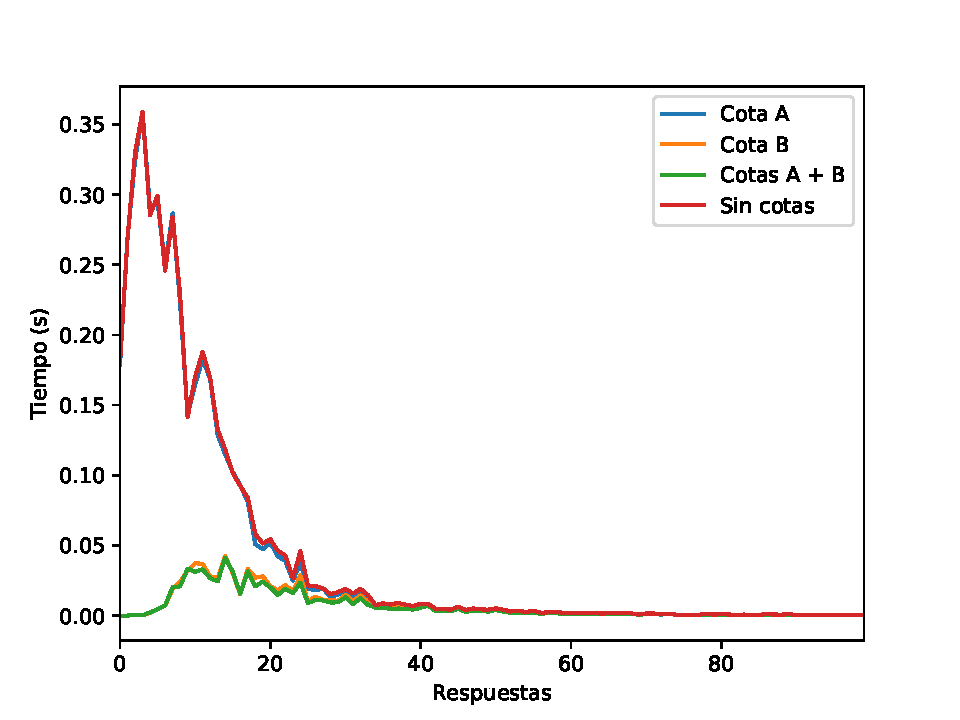
\includegraphics[scale=0.5]{Respuestas_st.pdf}
\end{figure}

Lo primero que se observa es la marcada diferencia que se produce al incorporar la poda B, tanto en tiempo como en comportamiento. La versión del algoritmo sin podas o con poda A obtiene los peores resultados cuando la cantidad de respuestas es menor a 5. Esto puede deberse a que al haber pocas opiniones, hay pocos agentes considerados poco confiables, y como consecuencia, hay conjuntos grandes de agentes que son consistentes. El algoritmo con poda B es particularmente rápido si encuentra un conjunto consistente grande tempranamente, ya que evita explorar ramas de menor profundidad al tamaño de este. Sin la poda B se deben recorrer una gran cantidad de ramas porque hay una cantidad pequeña de conjuntos inconsistentes. Por otro lado todas las variantes del algoritmo tienen un comportamiento similar cuando la cantidad de respuestas es mayor a 40. Se observa que el tiempo de ejecución disminuye significativamente. Esto probablemente se debe a que con un número tan alto de respuestas, existen muchos agentes catalogados como no confiables. Como consecuencia los conjuntos de agentes consistentes son pequeños y las ramas son cortadas rapidamente, lo cual conduce a que el tiempo de procesamiento disminuya. \\


%\begin{figure}[h]
%\caption{Tiempo en funcion de la cantidad de respuestas (Cotas A + B)}
%\centering
%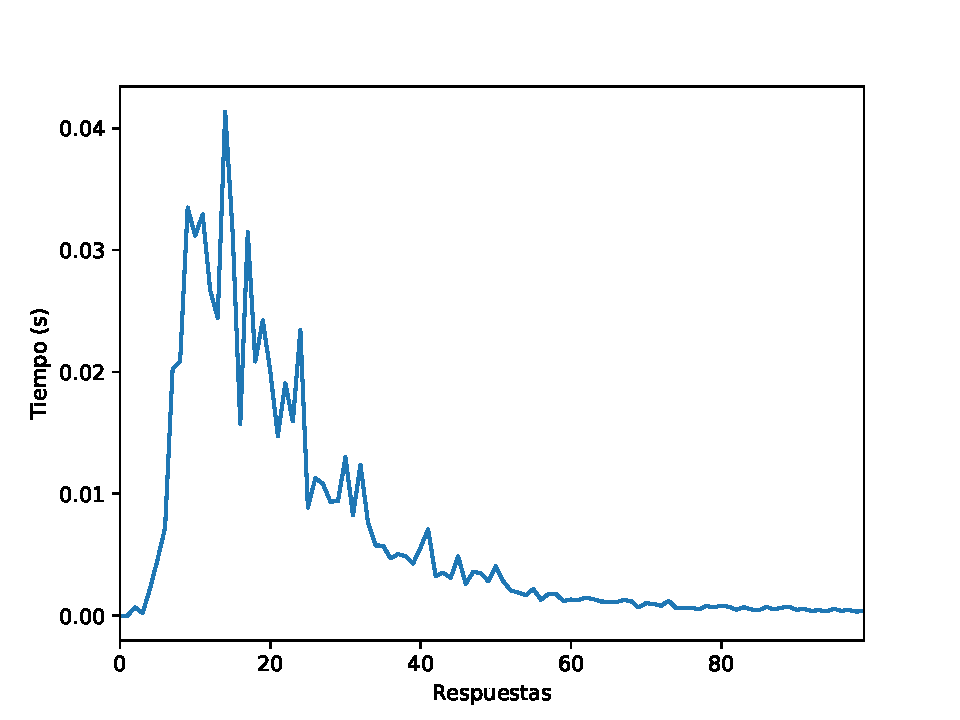
\includegraphics[scale=0.5]{Respuestas_AB_st.pdf}
%\end{figure}

\begin{figure}[h]
\caption{Tiempo en funcion de la cantidad de respuestas (casos)}
\centering
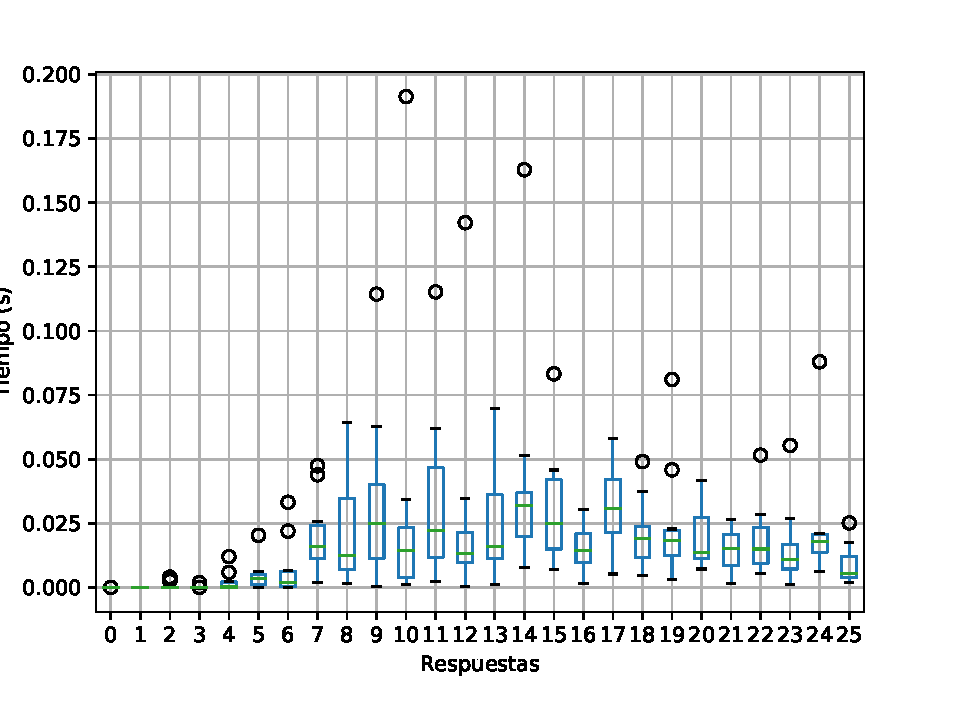
\includegraphics[scale=0.5]{Respuestas_box_st.pdf}
\end{figure}

En la figura 2 se muestra un diagrama de cajas del tiempo de ejecución en funcion de la cantidad de respuestas del algoritmo con ambas podas. Se observa que el pero caso, para una cantidad dada de respuestas, generalmente se encuentra muy alejado de la media. Esto permite concluir que más allá de la cantidad de respuestas, el significado particular del conjunto de respuestas tiene una gran influencia en el tiempo necesario para procesar el caso.

\subsection{Resultados variando la cantidad de agentes}

La figura 3 muestra los resultados obtenidos de variar la cantidad de agentes, manteniendo fijo la cantidad de respuestas en 20. Para cada configuración se crearon 10 casos. El valor graficado corresponde al tiempo promedio de los 10 casos, con el objetivo de evitar casos excepcionales sean tomados como representativos.

\begin{figure}[h]
\caption{Tiempo en funcion de la cantidad de agentes}
\centering
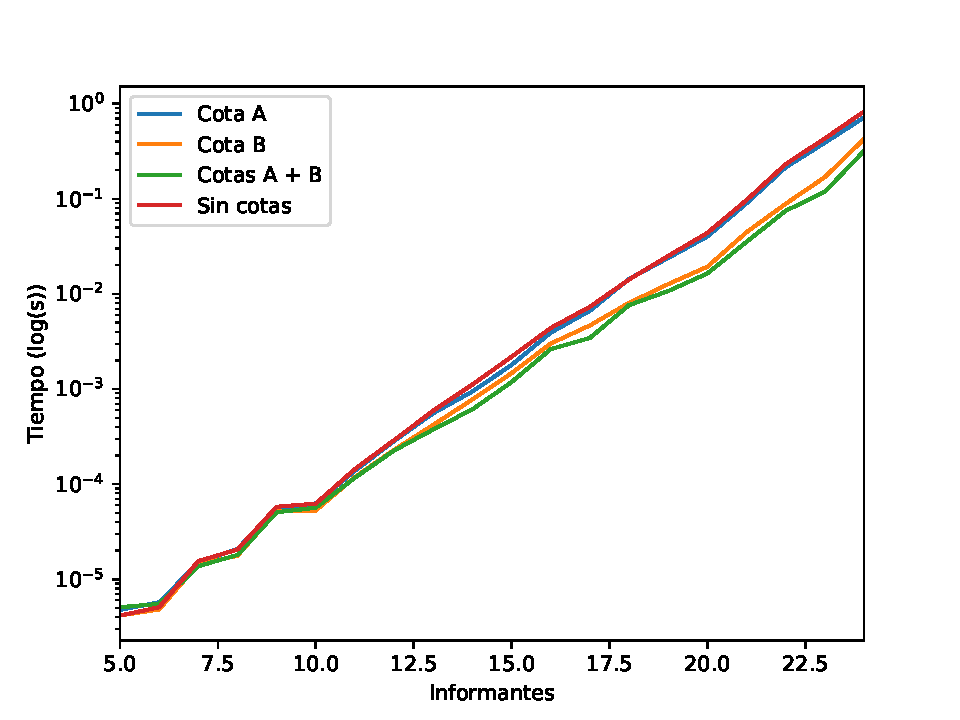
\includegraphics[scale=0.5]{Agentes_st.pdf}
\end{figure}

El eje temporal está en escala logarítmica, lo cual permite apreciar la naturaleza exponencial del algoritmo. 
Se observa que para casos con menos de 10 agentes, hay muy poca diferencia entre las distintas variantes del algoritmo.

\end{document}